\documentclass{article}
\usepackage{graphicx}
\title{Homework 3 \\ Alexandru Dumitrescu}
\date{}
\begin{document}
\maketitle
\section*{Task 2}

Heatmap for the constant epsilon: \\

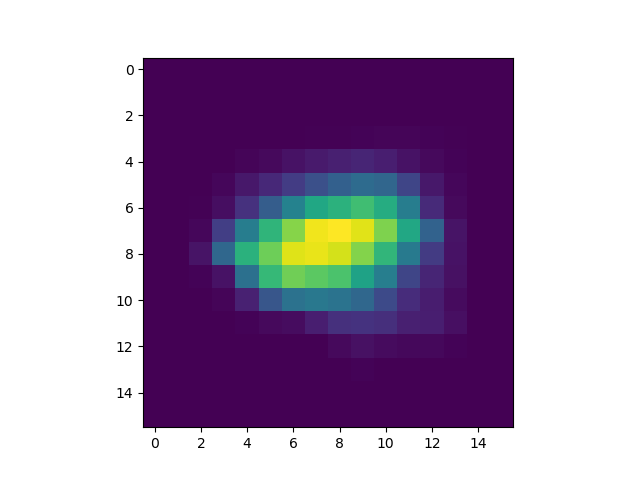
\includegraphics[scale=0.45]{constepsnormtraining.png} \\
Episode length over training steps for constant epsilon: \\

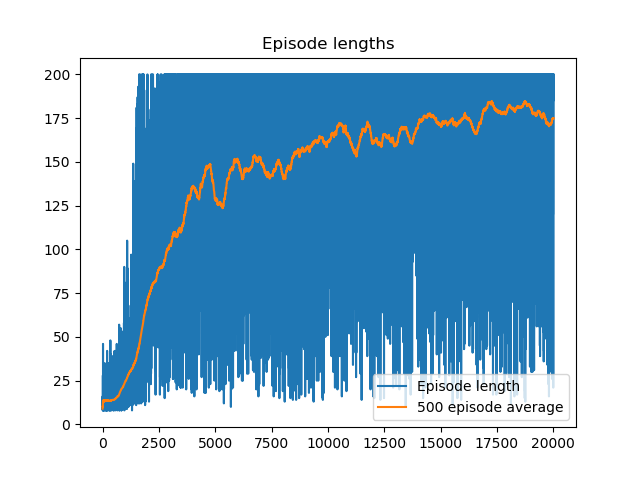
\includegraphics[scale=0.45]{constepsnormaltraining.png}\\
\newpage
Heatmap for glie with $a = \frac{20000}{9}$

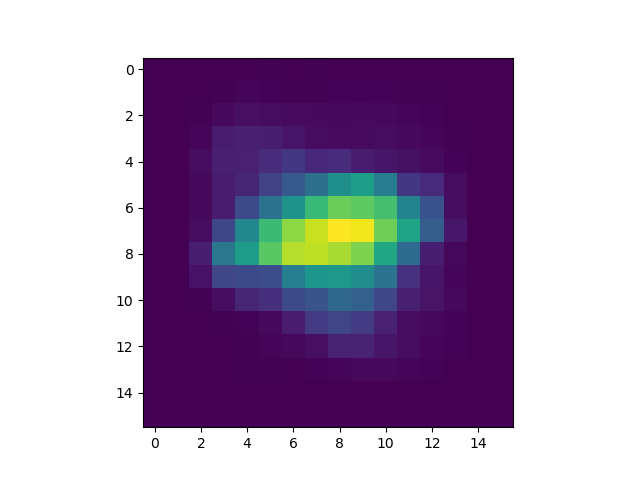
\includegraphics[scale=0.45]{glieepsnormtraining.png}\\

Episode length over training stepsfor glie with $a = \frac{20000}{9}$ \\


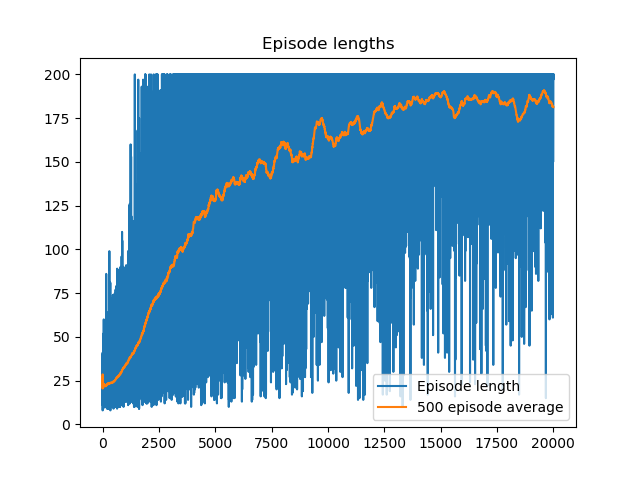
\includegraphics[scale=0.45]{glieepsnormaltraining.png}\\



\section{Question 1}
\subsection{a)}
The heatmap has 0s on all the states before the training, so it would have been uniformly dark.
\subsection{b)}
The initial state is never an instable one (the pole starts off being balanced). It will have one pixel where the reward is 1 and begin to lower this value as it goes in one of the directions. - episode is short, will update few action-vals.
\subsection{c)}
Fairly similar to the one when the training is finished. Also looking at the plot of training iterations, we can see how the trainig is more or less stabilized, so the heat-map must have decent enough (almost converged) values.
\section{Question 2}
\subsection{Q 2.1}
It should perform better when it is initialized with q\_initial=50:\\
Initializing with q\_init=50:
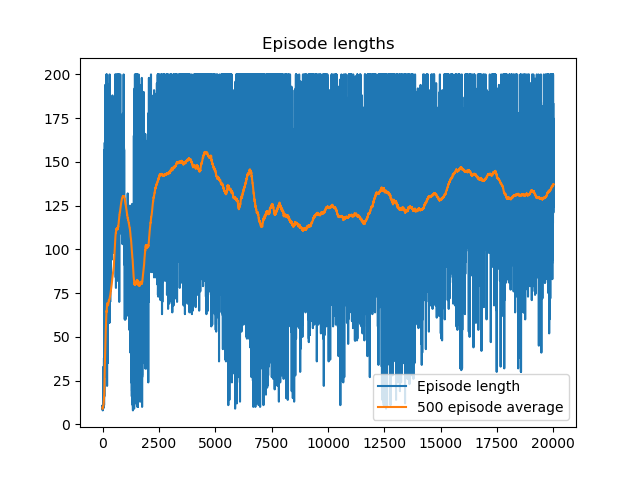
\includegraphics[scale=0.45]{50inittrainingiters.png}\\
Initializing with q\_init=0:
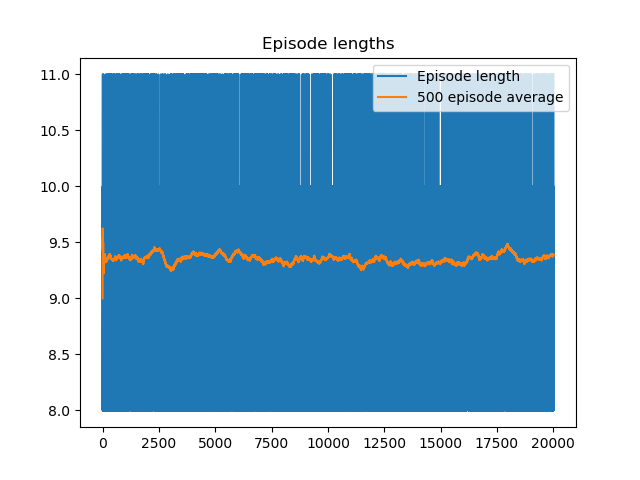
\includegraphics[scale=0.45]{0inittrainingiters.png}

\subsection{Q 2.2}

Everytime the model is in some state-action pair that fails, if q\_initial=50, that state-action will be updated using reward 0 (it will lower the Q\_value). This way, the next iteration, the model will avoid going to that state, since all other states are higher then the newly updated value in the one that it failed. This way, the model will explore all other states with value=50, whenever it finds some state-action that is bad.

\subsection{Q 2.3}
As explained above, the q\_grid will explore more when initialized with 50 because all never-visited state-action pairs will be all the time greater or equal to the ones already visited. When initializing with 0, however, the model will tend to take the same paths it has already taken, since all unvisited state-actions are all the time lower or equal to anything that it has already explored.

\section{Q 3}
\subsection{Q 3.1}
No, the maximum timesteps do increase, so it is able ot stay "alive" for longer, but that is not the goal of this problem.\\

The graph of cumulated rewards and 500 episode average can be seen below, which shows that the model isn't trainig anything useful:

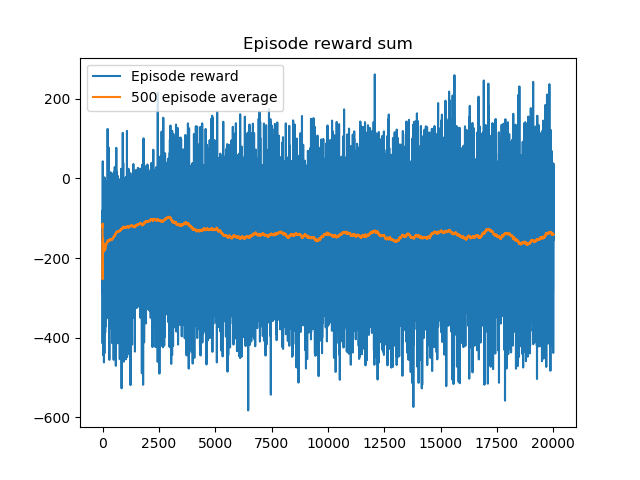
\includegraphics[scale=0.4]{lunar_lander_training_iter.png}

\subsection{Q 3.2}

The lunar lander has a huge 260milion state-action-space with a different setting - instead of being able to receive maximum rewards from the start, it now has to move through very many states until it finally finds something positive. Because it is so hard for it to randomly get to the landing point with so many state-action pairs(from the grid initialization, the only way to get to the positive-reward/landing point is randomly), it will be hard for it to achieve the final goal. 
\end{document}